\documentclass[12pt,compress,ngerman,utf8,t]{beamer}
\usepackage[ngerman]{babel}
\usepackage{calc}
\usepackage{ragged2e,wasysym,multicol}
\usepackage[protrusion=true,expansion=true]{microtype}

\graphicspath{{images/}}

\title[Superturingmaschinen]{Superturingmaschinen}
\author[Ingo Blechschmidt]{\textcolor{white}{Ingo Blechschmidt}}
\date[2016-10-04]{\vspace*{-4em}\ \\\textcolor{white}{\scriptsize Curry Club Augsburg \\ 4. Oktober 2016 und 3. November 2016}}

%\usetheme{Warsaw}
\useinnertheme[shadow=true]{rounded}
\useoutertheme{split}
\usecolortheme{orchid}
\usecolortheme{whale}
\setbeamerfont{block title}{size={}}

\useinnertheme{rectangles}

\usecolortheme{seahorse}
\definecolor{mypurple}{RGB}{150,0,255}
\setbeamercolor{structure}{fg=mypurple}
\definecolor{myred}{RGB}{150,0,0}
\setbeamercolor*{title}{bg=myred,fg=white}
\setbeamercolor*{titlelike}{bg=myred,fg=white}

\usefonttheme{serif}
\usepackage[T1]{fontenc}
\usepackage{libertine}

\newcommand{\M}{\mathcal{M}}
\newcommand{\R}{\mathrm{R}}
\newcommand{\NN}{\mathbb{N}}
\newcommand{\RR}{\mathbb{R}}
\newcommand{\Eff}{\mathrm{Eff}}
\newcommand{\TM}{\mathrm{TM}}
\newcommand{\STM}{\mathrm{STM}}
\newcommand{\RW}{\mathrm{RW}}

\newcommand{\slogan}[1]{%
  \begin{center}%
    \setlength{\fboxrule}{2pt}%
    \setlength{\fboxsep}{8pt}%
    {\usebeamercolor[fg]{item}\fbox{\usebeamercolor[fg]{normal text}\parbox{0.91\textwidth}{#1}}}%
  \end{center}%
}

\newcommand{\code}[1]{%
  \begin{center}%
    \setlength{\fboxrule}{1pt}%
    \setlength{\fboxsep}{8pt}%
    {\fbox{\parbox{0.81\textwidth}{#1}}}%
  \end{center}%
}

\newcommand{\explanation}[2]{
  #1 \\
  \qquad bedeutet: \\[0.4em]
  \qquad\qquad \begin{minipage}{0.84\textwidth}
  #2
  \end{minipage}
}

\newcommand{\explanationspoiler}[3]{
  \explanation{#1}{#2} \\[0.4em]
  \qquad\qquad\qquad #3
}

\setbeamertemplate{navigation symbols}{}

\setbeamertemplate{title page}[default][colsep=-1bp,rounded=false,shadow=false]
\setbeamertemplate{frametitle}[default][colsep=-2bp,rounded=false,shadow=false,center]

\newcommand{\hil}[1]{{\usebeamercolor[fg]{item}{\textbf{#1}}}}
\setbeamertemplate{frametitle}{%
  \vskip1em%
  \leavevmode%
  \begin{beamercolorbox}[dp=1ex,center]{}%
      \usebeamercolor[fg]{item}{\textbf{\textsf{\Large \insertframetitle}}}
  \end{beamercolorbox}%
}

\setbeamertemplate{footline}{%
  \leavevmode%
  \hfill%
  \begin{beamercolorbox}[ht=2.25ex,dp=1ex,right]{}%
    \usebeamerfont{date in head/foot}
    \insertframenumber\,/\,\inserttotalframenumber\hspace*{1ex}
  \end{beamercolorbox}%
  \vskip0pt%
}

\newcommand{\backupstart}{
  \newcounter{framenumberpreappendix}
  \setcounter{framenumberpreappendix}{\value{framenumber}}
}
\newcommand{\backupend}{
  \addtocounter{framenumberpreappendix}{-\value{framenumber}}
  \addtocounter{framenumber}{\value{framenumberpreappendix}}
}

\setbeameroption{show notes}
\setbeamertemplate{note page}[plain]

\begin{document}

% http://www.ufointernationalproject.com/wp-content/uploads/2015/11/a23.jpg
{\usebackgroundtemplate{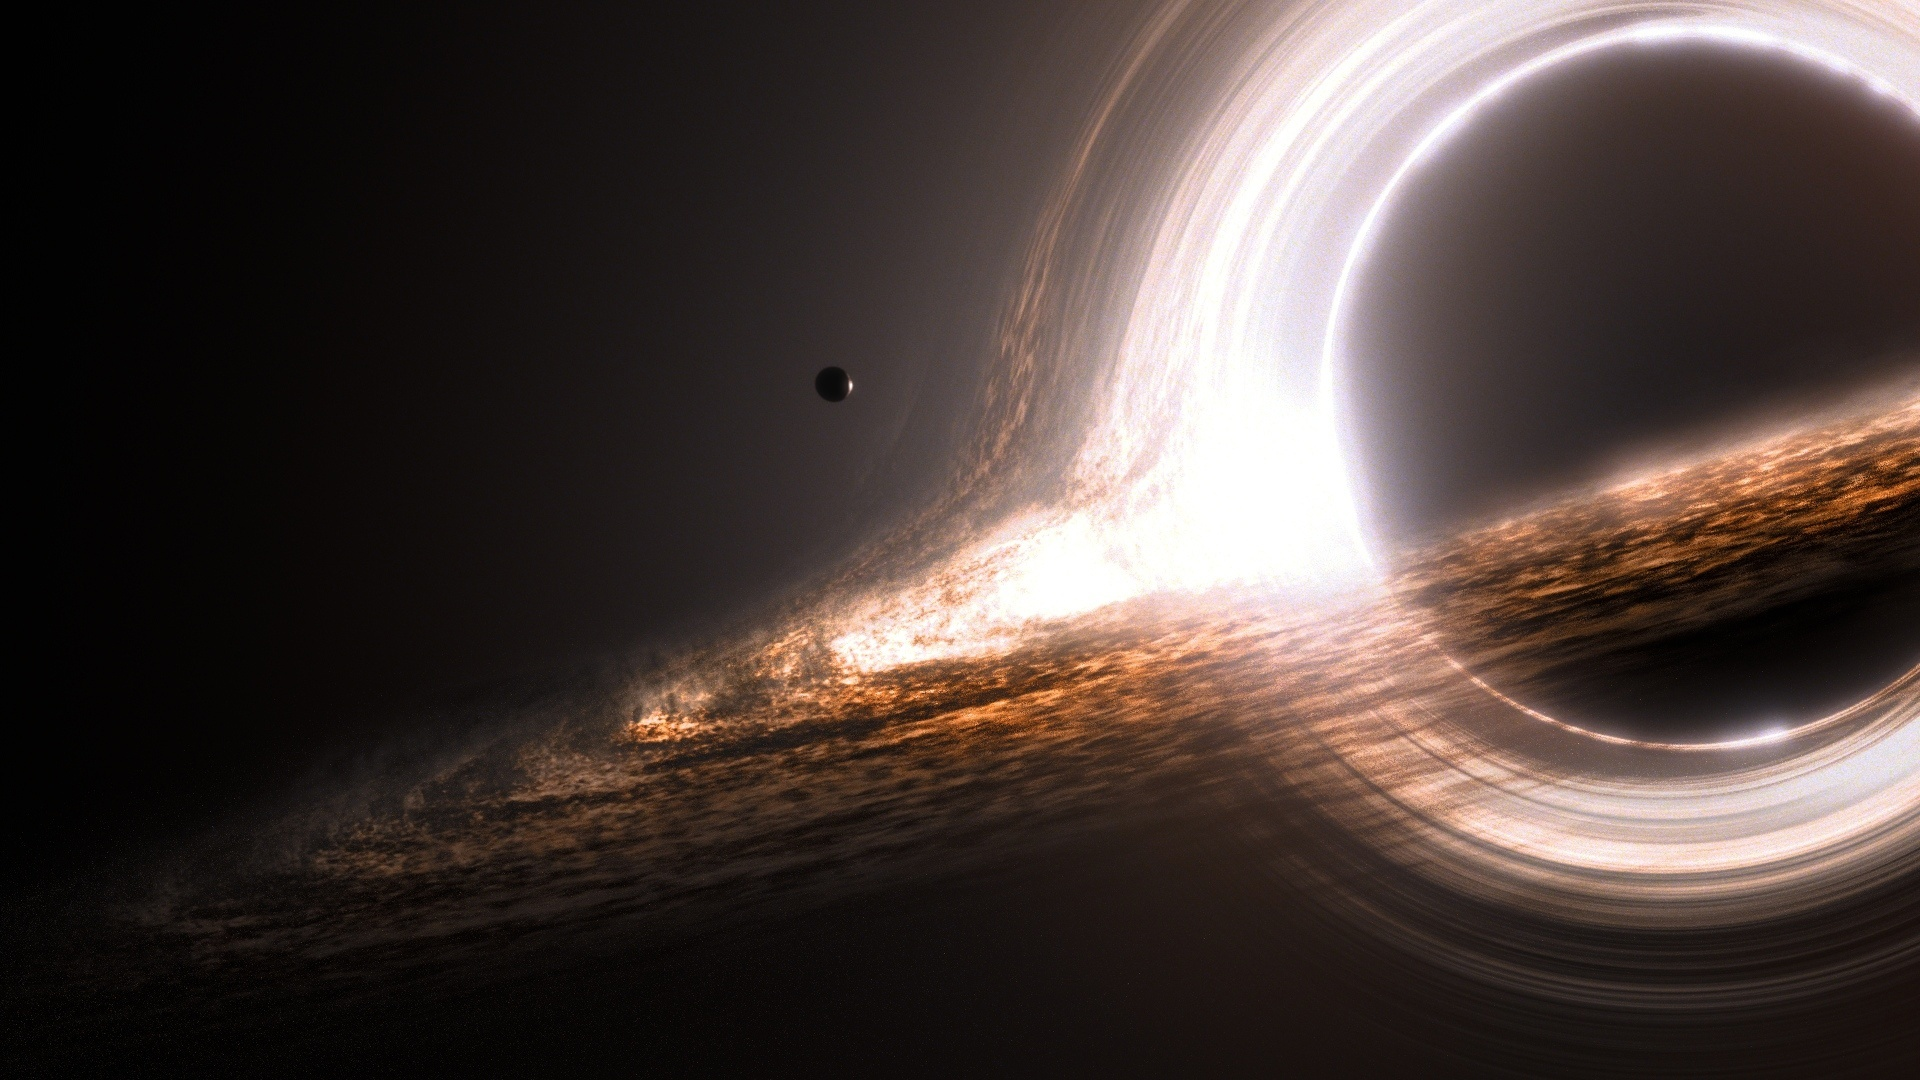
\includegraphics[height=\paperheight]{images/interstellar}}
\frame{\vspace*{12em}\titlepage}}
\frame{\tableofcontents}

\section{Erinnerungen}

\subsection{Gewöhnliche Turingmaschinen}

\begin{frame}{Ein Hoch auf Turingmaschinen}
  \begin{center}
    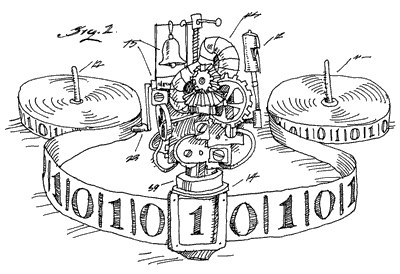
\includegraphics[width=0.6\textwidth]{images/turing-machine}
  \end{center}

  \begin{multicols}{2}
    \begin{enumerate}
      \item Schlichtheit
      \item Mechanischer Bezug
      \item Robustheit des Konzepts
      \item Äquivalenz zu anderen Modellen
      \item Querverbindungen
    \end{enumerate}
  \end{multicols}
\end{frame}
% mündlich: Es gibt Turingmaschinen mit 2 Zuständen und 4 Symbolen
% sowie mit 3 Zuständen und 3 Symbolen, deren Halteverhalten unbekannt ist.

\begin{frame}{Lustiges zu Turingmaschinen}
  \begin{enumerate}
    \item Schon kleine Turingmaschinen sind diffizil.
    \item Es gibt Turingmaschinen, deren Halteverhalten unabhängig von
    Standard-Axiomen der Mathematik ist.
    % Zum Beispiel: die TM, die nach einem Widerspruch in ZFC sucht.
    % Wenn ZFC konsistent ist, dann hält diese nicht.
    % Dieser Umstand ist aber nicht in ZFC beweisbar (Gödel II).
    \pause

    \item Alle sinnvollen Modelle für Berechenbarkeit stimmen für
    Funktionen~$\NN \to \NN$ überein.
    % Aber nicht für Funktionen höherer Ordnung!
    \pause

    \item Eine Menge ist genau dann rekursiv aufzählbar, wenn
    sie durch eine~$\Sigma_1$-Aussage definierbar ist:
    \[ \{ n \in \NN \,|\, \text{es gibt $m \in \NN$ mit $\heartsuit$} \}, \]
    \pause
    und wenn sie diophantisch ist:
    \[ \{ n \in \NN \,|\, \text{die Gl. $f(n,x_1,\ldots,x_m) = 0$
    besitzt eine Lösung} \}, \]
    wobei $f$ ein Polynom mit ganzzahligen Koeffizienten ist.
  \end{enumerate}
\end{frame}

\note{\justifying
  Eine~$\Sigma_1$-Aussage ist eine Aussage der Form
  \[ \text{"`Es gibt~$m \in \NN$ mit $\heartsuit$."',} \]
  wobei in der Teilaussage~$\heartsuit$ nur noch \emph{beschränkte
  Quantifikation} vorkommen darf -- also Formeln wie
  \[ \text{"`Für alle Zahlen kleiner als~$\cdots$ gilt \ldots"'} \]
  oder
  \[ \text{"`Es gibt eine Zahl kleiner als~$\cdots$ mit \ldots"'} \]
  und nicht Formeln wie
  \[ \text{"`Für alle Zahlen gilt \ldots"'} \]
  und
  \[ \text{"`Es gibt eine Zahl mit \ldots"'}. \]
  Die Teilaussage~$\heartsuit$ muss also in endlicher Zeit überprüfbar sein.\par
}


\subsection{Ordinalzahlen}

\begin{frame}{Ordinalzahlen messen Anordnung}
  \begin{center}
    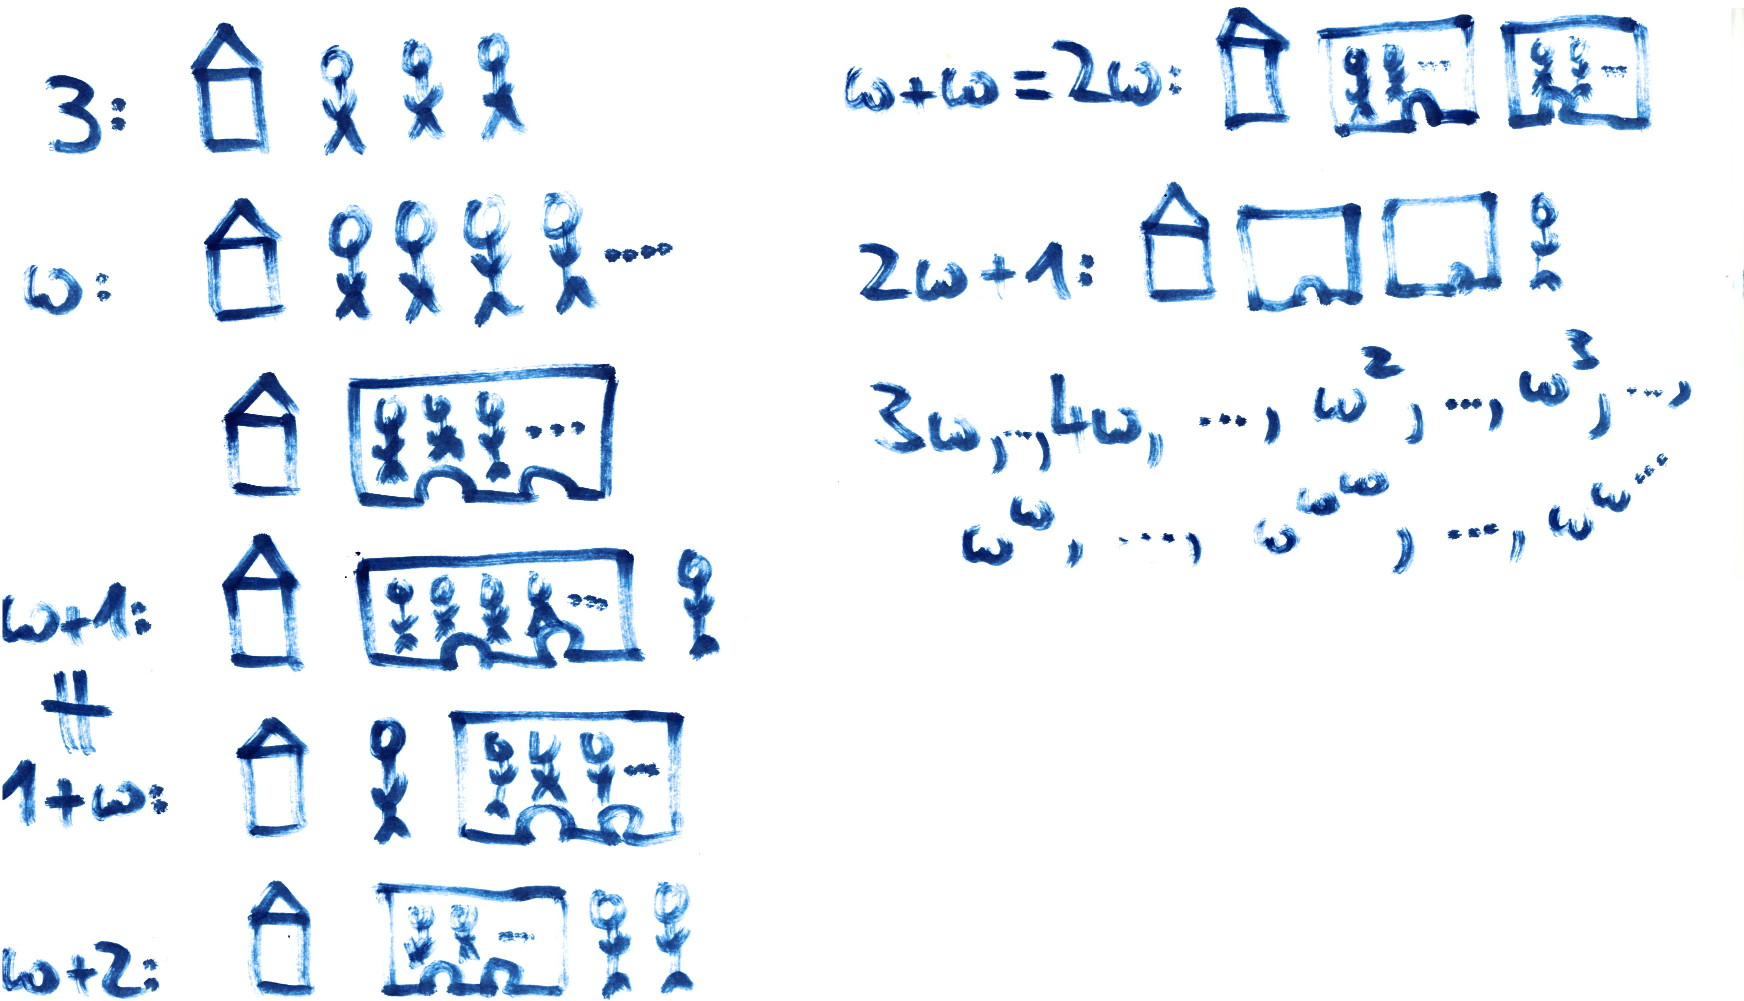
\includegraphics[width=\textwidth]{images/ordinal-intuition}
  \end{center}
\end{frame}

\note{\centering
  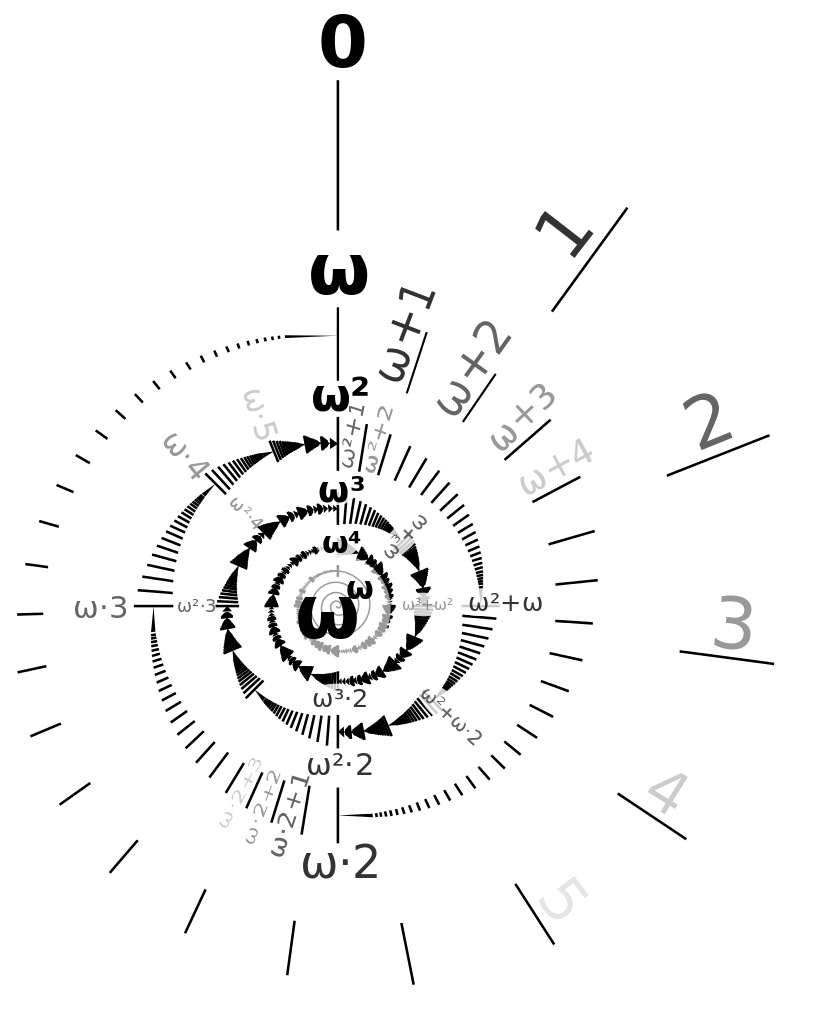
\includegraphics[width=0.7\textwidth]{images/ordinal-omega-omega}
  \par
}

\begin{frame}{Kardinalzahlen messen Anzahl}
  \begin{center}
    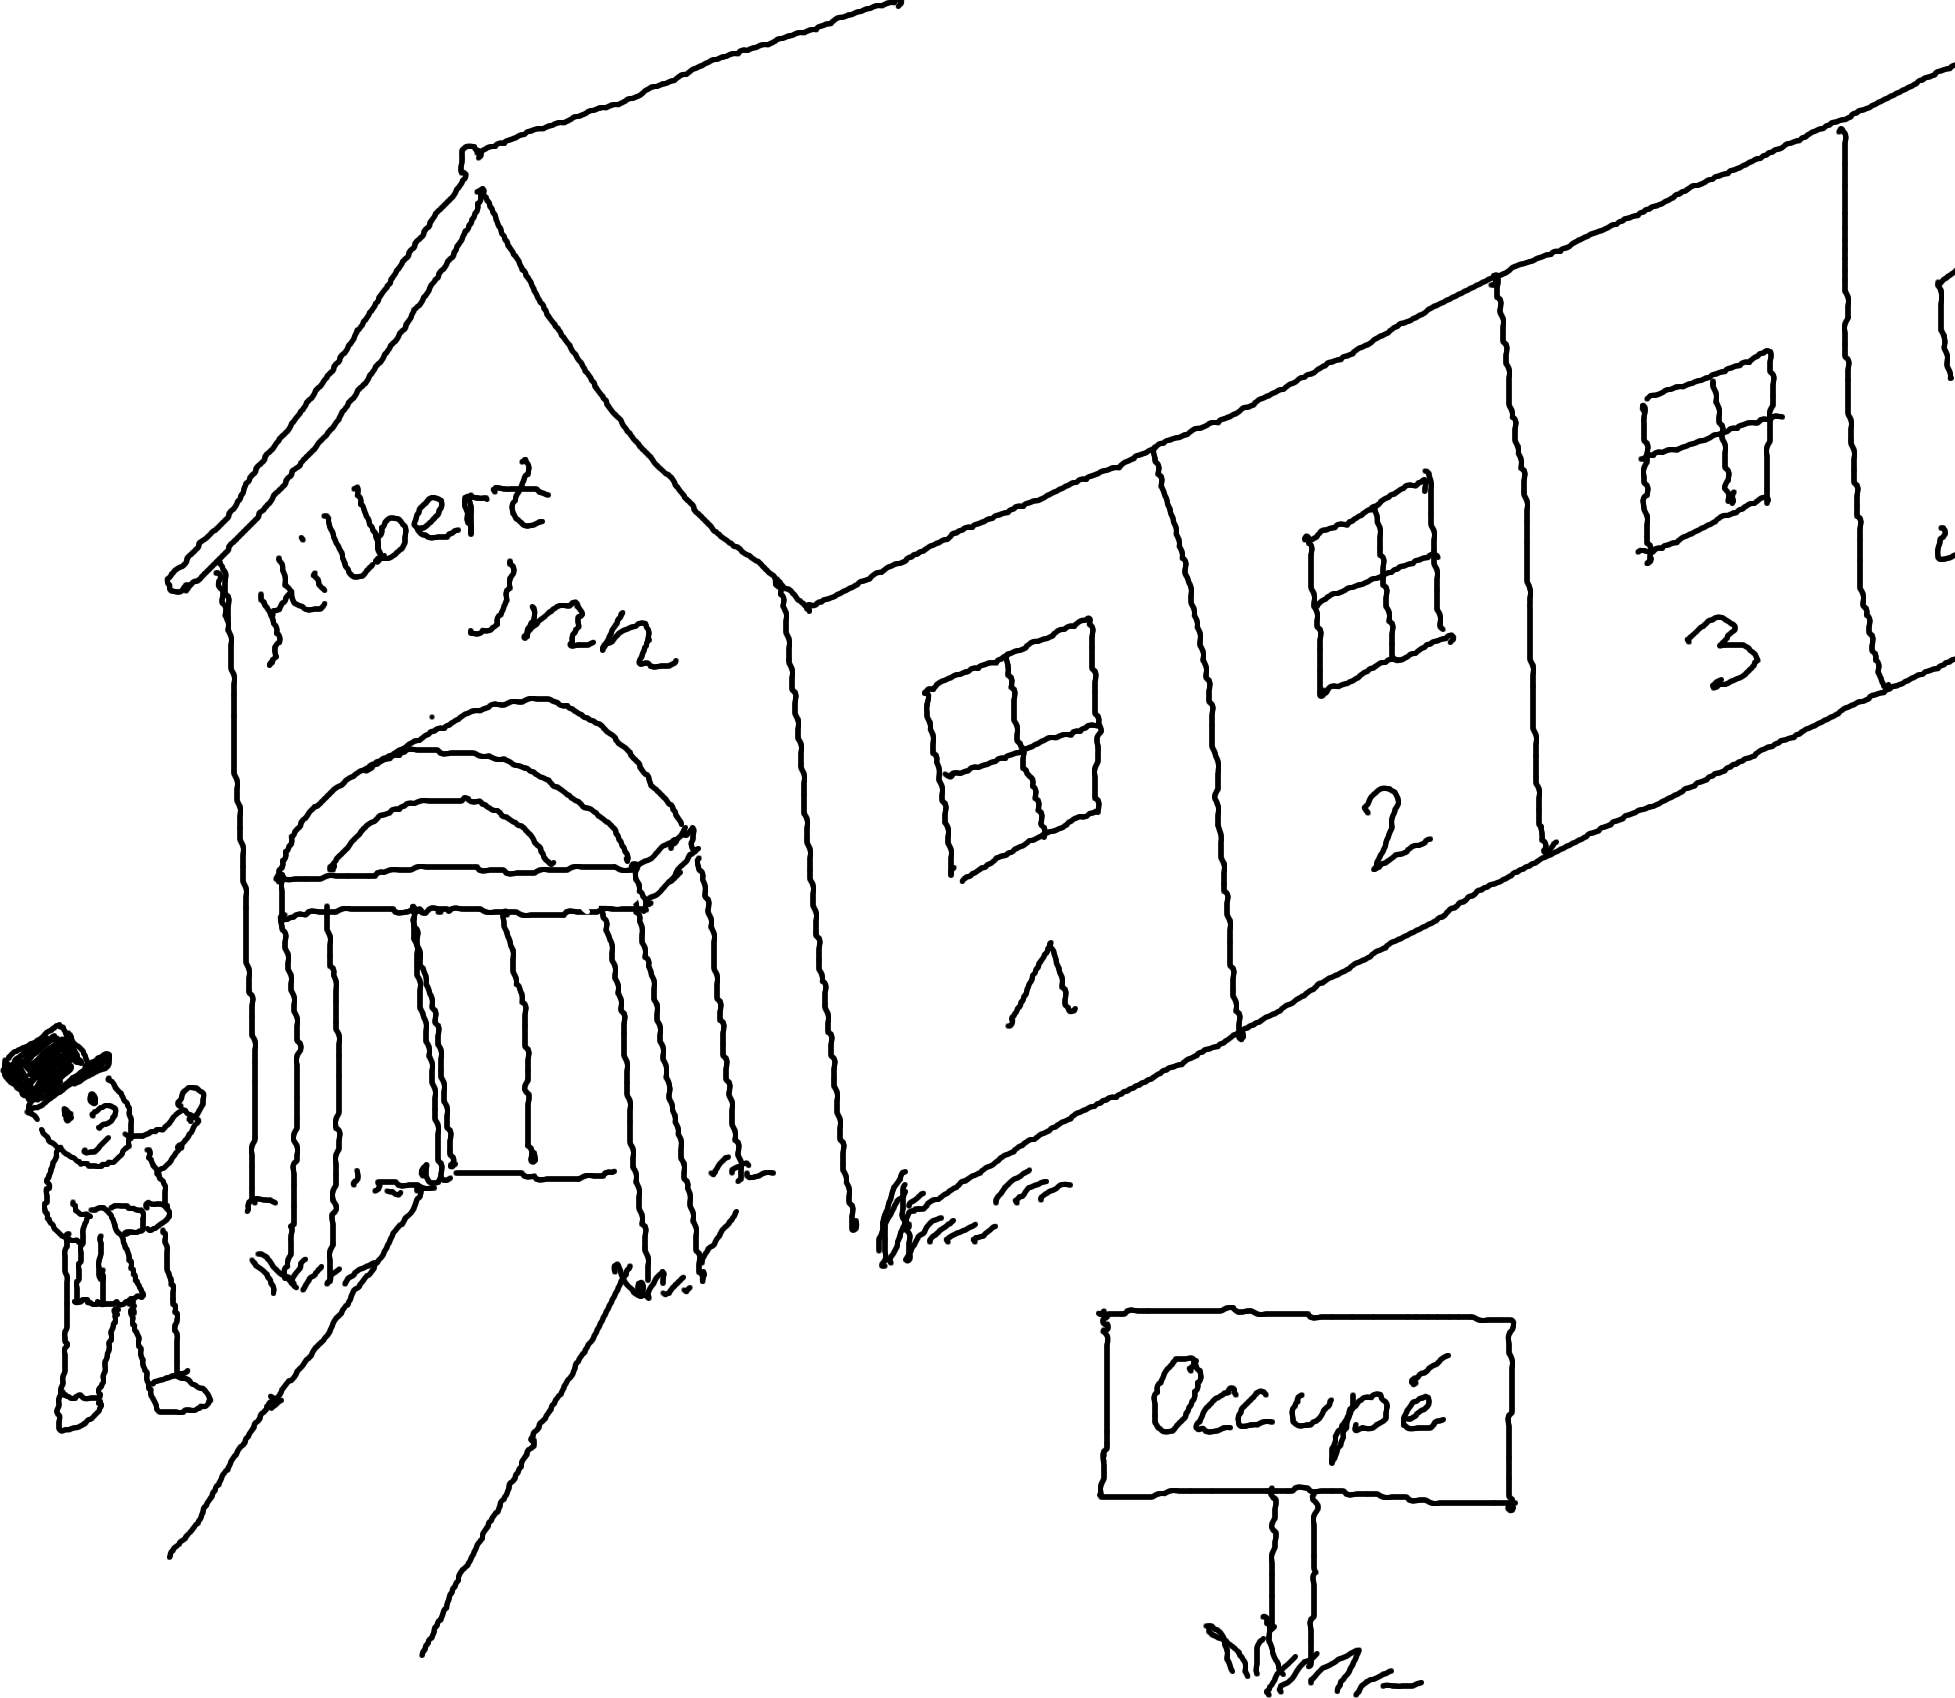
\includegraphics[width=0.5\textwidth]{images/hilberts-hotel}
  \end{center}

  \begin{itemize}
    \item Es gibt~$\aleph_0$ viele natürliche Zahlen.
    \pause
    \item $\aleph_0 + 1 = \aleph_0$, \quad
    \pause
    $\aleph_0 + \aleph_0 = \aleph_0$, \quad
    \pause
    $\aleph_0 \cdot \aleph_0 = \aleph_0$.
    \pause
    \item Es gibt mehr als~$\aleph_0$ viele reelle Zahlen.
  \end{itemize}
\end{frame}


\section[Grundlagen]{Grundlagen zu Superturingmaschinen}

\subsection{Erste Schritte}

\begin{frame}{Was sind Superturingmaschinen?}
  Bei Superturingmaschinen ist die Zeitachse spannender:
  \begin{itemize}
    \item normal: $0,\ 1,\ 2,\ \ldots$
    \item super:\phantom{rl} $0,\ 1,\ 2,\ \ldots,\ \omega,\ \omega + 1,\ \ldots,\ 2\omega,\ 2\omega
    + 1,\ \makebox[\widthof{R}][l]{$\ldots\ldots\ldots\ldots\ldots\ldots$}$
  \end{itemize}
  \bigskip

  Wird eine Limesordinalzahl erreicht, so wird
  \begin{itemize}
    \item die Maschine in einen designierten Zustand versetzt,
    \item der Schreib-/Lesekopf auf den Anfang bewegt und
    \item der "`lim sup"' aller vorherigen Bandinhalte genommen.
  \end{itemize}

  \begin{center}
    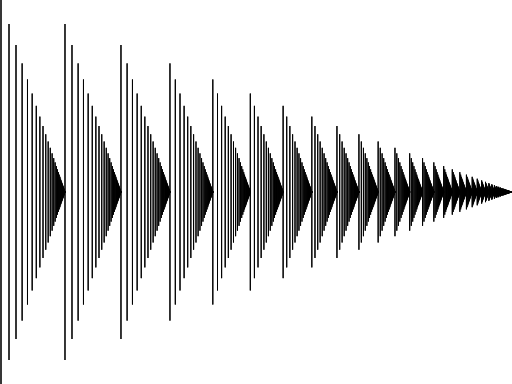
\includegraphics[width=0.35\textwidth]{images/ordinal-omega-squared}
  \end{center}
\end{frame}


\subsection[Fähigkeiten]{Fähigkeiten von Superturingmaschinen}

\begin{frame}{Was können Superturingmaschinen?}
  \begin{itemize}
    \item Alles, was gewöhnliche Turingmaschinen können.
    \item Zahlentheoretische Behauptungen überprüfen:
      \begin{itemize}
        \item $\forall$ -- "`Für alle Zahlen gilt \ldots"'    % omega
        \item $\exists$ -- "`Es gibt eine Zahl mit \ldots"'   % omega
        \item $\forall\,\exists$ -- "`Für alle Zahlen~$n$
        gibt es jeweils eine Zahl~$m$ mit \ldots"'            % 2 omega
        \item $\exists\,\forall$ -- "`Es gibt eine Zahl~$n$,
        sodass für alle Zahlen~$m$ gilt: \ldots"'             % omega
        \item $\forall\,\exists\,\forall$,                    % omega^2
        $\exists\,\forall\,\exists$, \ldots
      \end{itemize}
    \item Entscheiden, ob gewöhnliche Turingmaschinen halten.
    \item \ \\[-1.2em]\mbox{Superturingmaschinen und verwandte Maschinen simulieren.}
    \item $\Pi_1^1$- und $\Sigma_1^1$-Aussagen entscheiden.
  \end{itemize}
  \pause

  \hil{Aber:} Superturingmaschinen können nicht alle Funktionen berechnen
  und nicht jede 0/1-Folge aufs Band schreiben.
  % Es gibt~$2^{\aleph_0}$ viele Funktionen $\NN \to \NN$, aber nur $\aleph_0$
  % viele Superturingmaschinen.
\end{frame}

\begin{frame}{Fundierung von Bäumen}
  Ein Baum ist genau dann \hil{fundiert}, wenn er keinen unendlichen Pfad enthält.

  \begin{center}
    \scalebox{0.4}{\input{images/nonwellfounded-tree.pdf_t}}
  \end{center}

  Superturingmaschinen können die Fundiertheit von Bäumen entscheiden.
\end{frame}

\begin{frame}{Ein kleines Wunder}
  Superturingmaschinen können~$\Pi_1^1$- und $\Sigma_1^1$-Aussagen entscheiden:
  \[ \text{"`Für jede Funktion~$\NN \to \NN$ gilt \ldots"'} \]
  \[ \text{"`Es gibt eine Funktion~$\NN \to \NN$ mit \ldots"'} \]

  \vspace*{0.5em}
  Und das, obwohl es überabzählbar viele Funktionen~$\NN \to \NN$ gibt, aber
  Superturingmaschinen nur ein abzählbares Band verwenden und (nächste
  Folie) immer schon nach abzählbar vielen Schritten halten
  oder in Endlosschleifen geraten.
\end{frame}


\subsection[Laufzeit]{Laufzeit von Superturingmaschinen}

\begin{frame}{Wann halten Superturingmaschinen?}
  Schon nach \hil{abzählbar vielen} ($\leq \aleph_0$ vielen) Schritten hält jede
  Superturingmaschine entweder an oder wiederholt sich.
  \bigskip
  \pause

  \emph{Sprechweise.} Eine Ordinalzahl ist genau dann \hil{abzählbar}, wenn sie
  nur abzählbar viele Vorgänger hat.
  \bigskip

  Genau die abzählbaren Ordinalzahlen lassen sich in~$\RR$ einbetten.

  \begin{center}
    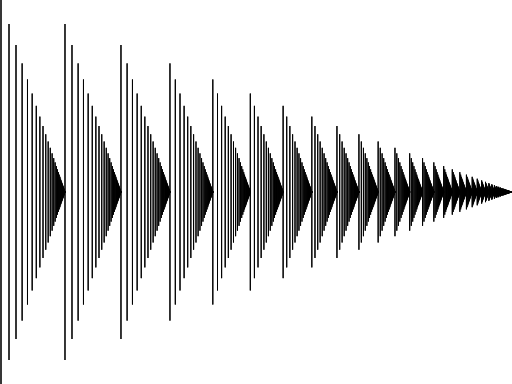
\includegraphics[width=0.35\textwidth]{images/ordinal-omega-squared}
  \end{center}
\end{frame}

\note{
  \emph{Notation.} Es ist~$\omega_1$ die erste Ordinalzahl, vor der
  \emph{überabzählbar} unendlich viele Ordinalzahlen kommen.
  \bigskip

  \emph{Behauptung.}
  Hat eine Superturingmaschine nach \emph{abzählbar vielen} Schritten noch
  nicht angehalten, so hält sie nie.
  \bigskip

  \justifying
  \emph{Beweis.} Angenommen, eine Superturingmaschine hat vor
  Schritt~$\omega_1$ noch nicht gehalten. Dann gibt es eine
  Ordinalzahl~$\alpha_0 < \omega_1$, zu der sich alle Zellen, die sich bis
  vor~$\omega_1$ stabilisieren werden, schon stabilisiert haben. Ferner gibt es
  Ordinalzahlen
  \[ \alpha_0 < \alpha_1 < \alpha_2 < \cdots < \omega_1, \]
  sodass sich zwischen~$\alpha_n$ und~$\alpha_{n+1}$ all die Zellen, die sich
  bis~$\omega_1$ noch ändern werden, jeweils mindestens einmal ändern.
  Sei~$\delta = \lim_{n \to \infty} \alpha_n$. Das ist eine Ordinalzahl~$<
  \omega_1$, also eine abzählbare Ordinalzahl. Dann ist die Aufnahme der
  Superturingmaschine bei~$\delta$ gleich der bei~$\omega_1$. Die
  Superturingmaschine wiederholt sich also.
  \par
}


\section{Besondere Phänomene}

\subsection[Wiederholungen]{Ausbrechen aus Wiederholungen}

\begin{frame}{Ausbrechen aus Wiederholungen}
  Was macht folgende Superturingmaschine?

  \code{Prüfe im Start- und Limeszustand, ob die aktuelle Zelle eine Eins enthält.
  \begin{itemize}
    \item Wenn ja, dann halte.
    \item Wenn nein, dann lass die Zelle aufleuchten und laufe ohne Unterlass nach
    rechts.
  \end{itemize}}
  \pause

  Sie scheint sich zu wiederholen, hält aber nach Schritt~$\omega^2$.
  \bigskip
  \pause

  Eine Superturingmaschine wiederholt sich genau dann, wenn
  \begin{itemize}
    \item die Aufnahmen zu zwei
    Limesordinalzeiten gleich sind und
    \item zwischen diesen Zeiten keine Zellen, die
    Null waren, zu Eins werden.
  \end{itemize}
\end{frame}


\subsection{Stempelbare Ordinalzahlen}

\begin{frame}{Stempelbare Ordinalzahlen}
  Eine Ordinalzahl~$\alpha$ ist genau dann \hil{stempelbar} (clockable),
  falls es eine Superturingmaschine gibt, die genau nach Schritt~$\alpha$ hält.

  \only<1>{\begin{itemize}
    \item Jede endliche Ordinalzahl ist stempelbar.
    \item Stempelbar sind außerdem: $\omega$, $2\omega$, $\omega^2$
    \item Sind~$\alpha$ und~$\beta$ stempelbar, so auch~$\alpha+\beta$
    und~$\alpha \cdot \beta$.
    \item Nur abzählbar viele Ordinalzahlen sind stempelbar.
    \item Jede rekursive Ordinalzahl ist stempelbar.
  \end{itemize}}

  \only<2>{
    \begin{block}{Beschleunigungssatz}
    Ist~$\alpha + n$ stempelbar, so auch~$\alpha$.
    \end{block}

    \begin{block}{Große-Lücken-Satz}
    Für jede stempelbare Ordinalzahl~$\alpha$
    gibt es eine Lücke der Länge~$\geq \alpha$ in den stempelbaren Ordinalzahlen.
    \end{block}

    \begin{block}{Viele-Lücken-Satz}
    Ist~$\alpha$ eine schreibbare Ordinalzahl,
    so gibt es mindestens~$\alpha$ viele Lücken der Länge~$\geq \alpha$ in den
    stempelbaren Ordinalzahlen.
    \end{block}
    % Lückenlose-Blöcke-Satz?
  }
\end{frame}

\note{\justifying
  Kurioserweise gibt es auch den \emph{Lückenlose-Blöcke-Satz} (Gapless Blocks
  Theorem): Es gibt in den Ordinalzahlen "`lange Abschnitte"' von lauter
  stempelbaren Ordinalzahlen.
  \par
}

\begin{frame}{Erinnerung: Diagonalisierung}
  \begin{center}
    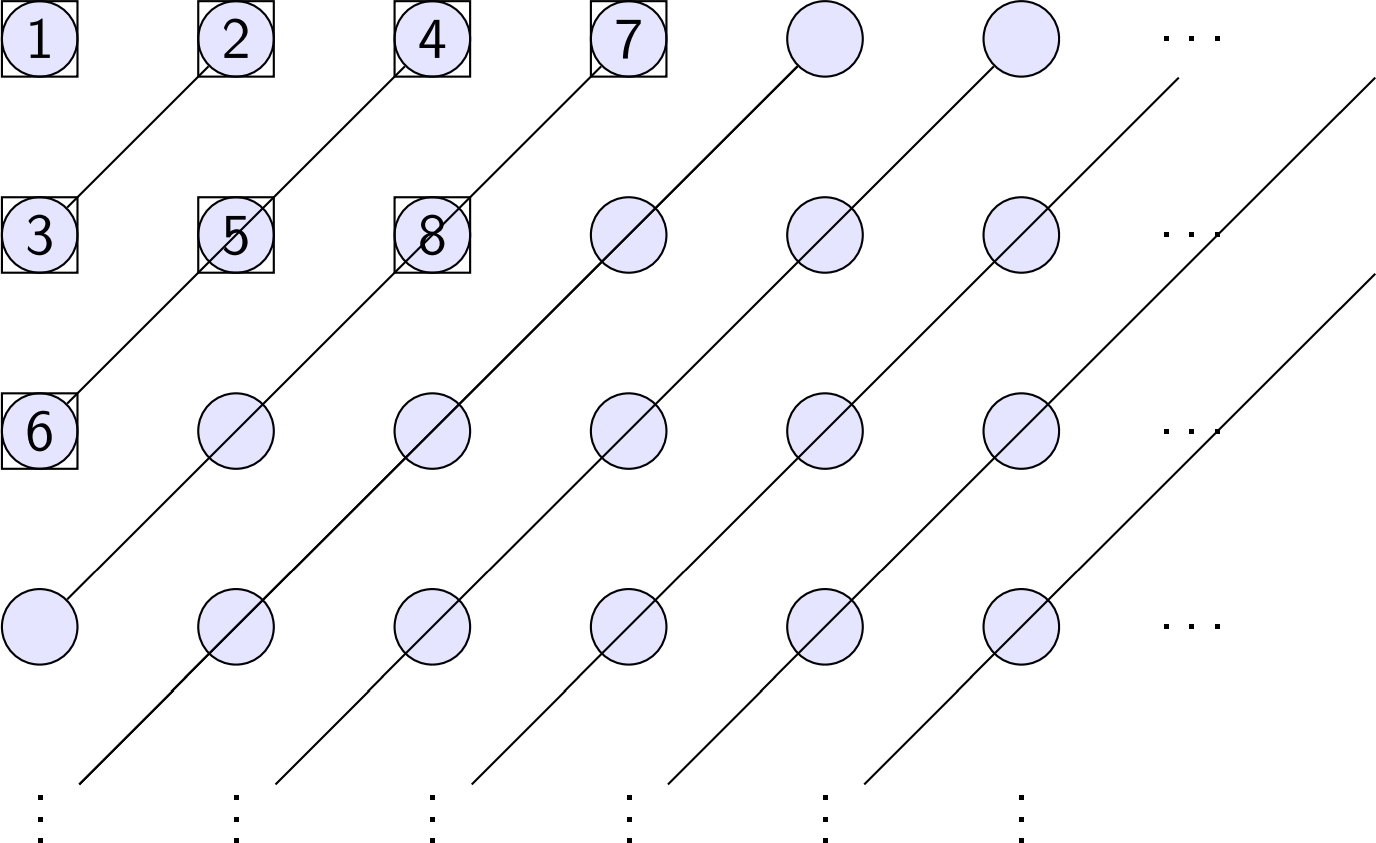
\includegraphics[width=0.8\textwidth]{images/diagonalization}
  \end{center}
\end{frame}

\begin{frame}{Lückenexistenzsatz}
  \mbox{Die erste Lücke nach jeder stempelbaren Ordinalzahl hat
  Länge~$\omega$.}
  \bigskip

  \vspace*{-1.2em}
  \justifying
  \emph{Beweis.} Sei~$\alpha$ eine stempelbare Ordinalzahl.
  Sei~$\beta$ die kleinste nicht-stempelbare Ordinalzahl nach~$\alpha$.
  Dann gibt es keine stempelbaren Ordinalzahlen zwischen~$\beta$ und~$\beta +
  \omega$. Und~$\beta + \omega$ selbst ist stempelbar durch folgendes Programm:
  \code{
    Simuliere alle Superturingmaschinen auf verzahnte Art und Weise.
    Behalte dabei insbesondere das Programm im Auge, das nach Schritt~$\alpha$
    halten wird. Sobald dieses gehalten hat, simuliere so lange weiter, bis der
    Zeitpunkt~$\beta$ erreicht ist, zu dem keine Superturingmaschine hält, und halte
    dann.}
  Zur Erkennung waren aber noch~$\omega$ Schritte nötig.
\end{frame}


\subsection{Lost-Melody-Theorem}

\begin{frame}{Lost-Melody-Theorem}
  Es gibt Bandinhalte, die
  \begin{itemize}
    \item Superturingmaschinen nicht schreiben, aber
    \item erkennen können.
  \end{itemize}
  \pause
  \bigskip

  \emph{Beweis.} Sei~$c$ eine Kodierung aller Ablauf{}folgen aller
  Superturingmaschinen als unendliche 0/1-Folge.
  \begin{itemize}
    \item Dann ist~$c$ nicht schreibbar.
    \item Aber~$c$ ist erkennbar.
  \end{itemize}

  \hfill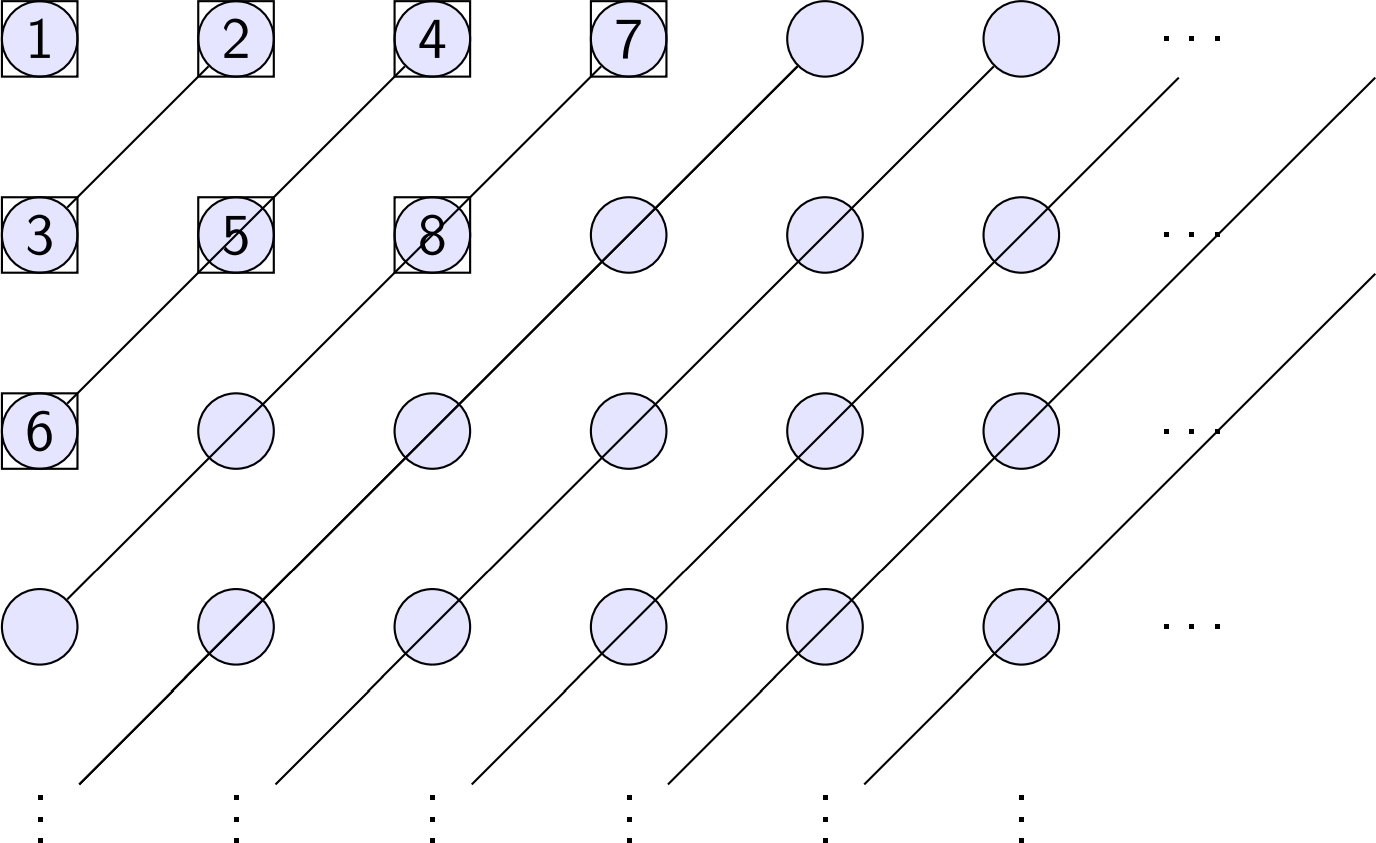
\includegraphics[width=0.4\textwidth]{images/diagonalization}
\end{frame}


\section[Effektive Topoi]{Der effektive Topos}

\subsection[Alternativuniversen]{Mathematische Alternativuniversen}

\begin{frame}{Mathematische Alternativuniversen}
  \justifying
  Zu jedem Rechenmodell~$\M$ gibt es einen
  \hil{Topos}~$\Eff(\M)$, in den wir mit \hil{Realisierbarkeitstheorie}
  hineinschauen können.
  \bigskip
  \pause

  \explanation{$\Eff(\TM) \models \text{"`Für jede Zahl~$n$ gibt es eine
  Primzahl~$p > n$."'}$}{Es gibt eine Turingmaschine, die eine Zahl~$n$ vom Band einliest
  und eine Primzahl~$p > n$ als Ausgabe aufs Band schreibt.}
  \bigskip

  \explanation{$\Eff(\TM) \models \text{"`Jede Zahl besitzt eine
  Primfaktorzerlegung."'}$}{Es gibt eine Turingmaschine, die eine Zahl~$n$ vom
  Band einliest und eine Liste von Primzahlen, deren Produkt~$n$ ist, aufs Band
  schreibt.}
\end{frame}


\subsection[Intuitionistische Logik]{Das Wunder intuitionistischer Logik}

\begin{frame}{Was gilt in Alternativuniversen?}
  \hil{Metatheorem:} Jede Aussage, die sich \hil{intuitionistisch} beweisen
  lässt, gilt in allen Topoi.
  \bigskip

  {\centering
  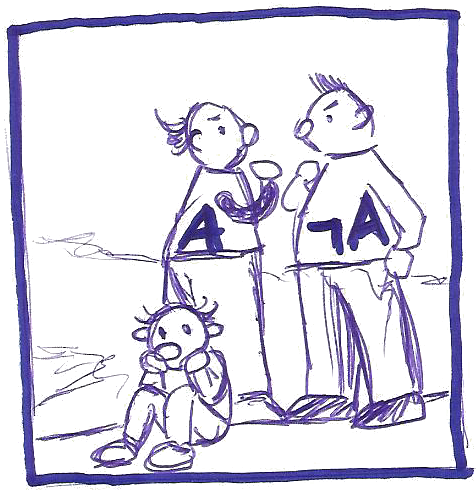
\includegraphics[width=0.2\textwidth]{images/lem}
  \par}

  \begin{block}{Schon gewusst?}
    Intuitionistische Logik ist wie klassische Logik, nur ohne:
    \begin{itemize}
      \item Axiom vom ausgeschlossenen Dritten (LEM): $\varphi \vee \neg\varphi$
      \item Axiom der Doppelnegationselimination (DNE): $\neg\neg\varphi \Rightarrow \varphi$
    \end{itemize}
    So sind Widerspruchsbeweise nicht pauschal möglich.
  \end{block}

  %\explanation{$\Eff(\TM) \models \varphi \vee \neg\varphi$}{Es gibt eine
  %Turingmaschine, die entweder einen Zeugen von~$\varphi$ oder einen Zeugen
  %von~$\neg\varphi$ berechnet.}
\end{frame}


\subsection[Tautologien]{Effektive Bedeutung klassischer Tautologien}

\begin{frame}{LEM für Gleichheit von Funktionen}
  \explanationspoiler{$\Eff(\TM) \models \begin{minipage}[t]{0.7\textwidth}
  "`Für jede Funktion~$f : \NN \to \NN$ gilt: Entweder ist~$f$ die Nullfunktion
  oder nicht."'\end{minipage}$}{Es gibt eine Turingmaschine, die eine Kodierung
  einer Turingmaschine~$M$, welche eine Funktion $\NN \to \NN$ berechnet, als
  Eingabe vom Band liest und dann entscheidet, ob~$M$ stets Null als Ausgabe
  produziert oder nicht.}{Das stimmt nicht.}
  \bigskip
  \pause

  \emph{Bemerkung:} Aus externer Sicht ist das Objekt~$\NN^\NN$ des effektiven
  Topos die Menge der \hil{berechenbaren} Funktionen.
  \bigskip
  \pause

  In~$\Eff(\STM)$ stimmt die Aussage.
\end{frame}

\begin{frame}{LEM fürs Halten von Turingmaschinen}
  \explanationspoiler{$\Eff(\TM) \models \text{"`Jede Turingmaschine~$M$ hält
  oder hält nicht."'}$}{Es gibt eine Turingmaschine, die die Kodierung einer
  Turingmaschine~$M$ als Eingabe vom Band liest und dann entscheidet, ob~$M$
  hält oder nicht.}{Das stimmt nicht.}
  \bigskip
  \pause

  In~$\Eff(\STM)$ stimmt die Aussage.
\end{frame}

\begin{frame}{Markovs Prinzip}
  \explanationspoiler{$\Eff(\TM) \models \begin{minipage}[t]{0.7\textwidth}
  "`Für jede Funktion~$f : \NN \to \NN$, welche nicht die Nullfunktion ist,
  gibt es eine Stelle~$n \in \NN$ mit~$f(n) \neq 0$."'\end{minipage}$}{Es gibt
  eine Turingmaschine, die eine Kodierung einer Turingmaschine~$M$, welche eine
  Funktion $\NN \to \NN$ und zwar nicht die Nullfunktion berechnet, als Eingabe
  vom Band liest und dann eine Zahl~$n$ aufs Band schreibt, sodass~$M$ bei
  Eingabe von~$n$ nicht Null aufs Band schreibt.}{Das stimmt! (Unbeschränkte
  Suche.)}
\end{frame}

\begin{frame}{Church--Turing-These}
  \justifying
  Die \hil{Church--Turing-These} besagt: Lässt sich eine Funktion~$f : \NN \to
  \NN$ in der "`realen Welt berechnen"', so gibt es eine Turingmaschine,
  die~$f$ berechnet.
  \bigskip

  \explanationspoiler{$\Eff(\TM) \models \begin{minipage}[t]{0.7\textwidth}
  "`Jede Funktion~$f : \NN \to \NN$ lässt sich durch eine Turingmaschine
  berechnen."'\end{minipage}$}{Es gibt eine Turingmaschine, die eine Kodierung
  einer Turingmaschine~$M$, welche eine Funktion~$f : \NN \to \NN$ berechnet, als
  Eingabe vom Band liest und dann die Kodierung einer Turingmaschine,
  welche~$f$ berechnet, aufs Band schreibt.}{Das ist trivial! "`cat"' ist die
  gesuchte Maschine.}
  \bigskip
  \pause

  In~$\Eff(\STM)$ und~$\Eff(\lambda)$ stimmt die Aussage nicht.
\end{frame}

\begin{frame}{Automatische Stetigkeit}
  \justifying
  Im üblichen Universum stimmt folgende Aussage \hil{nicht}:
  \[ \text{"`Jede Funktion~$f : \RR \to \RR$ ist stetig."'} \]
  Eine Funktion~$f$ heißt genau dann \hil{stetig}, falls für jede Zahl~$x$ zur
  Bestimmung von endlich vielen Nachkomma\-stel\-len von~$f(x)$ schon
  endlich viele Nachkommastellen von~$x$ genügen.\par

  \centering
  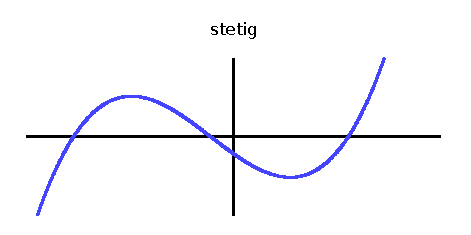
\includegraphics[width=0.5\textwidth]{images/plot-1}
  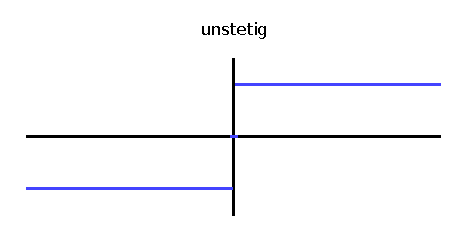
\includegraphics[width=0.5\textwidth]{images/plot-2}
  \par
  \pause

  \justifying
  Stimmt in~$\Eff(\TM)$. \pause
  Stimmt in~$\Eff(\RW)$, falls black boxes und private Kommunikationskanäle
  möglich sind und in endlicher Zeit nur endlich viele Rechenschritte
  ausgeführt werden können.
  \par
\end{frame}

\begin{frame}{Seltsame Größenverhältnisse}
  \only<1-2>{
    Es gibt keine Surjektion~$\NN \to \NN^\NN$; die Menge~$\NN^\NN$ der
    Funktionen~$\NN \to \NN$ ist viel größer als~$\NN$.
    \bigskip

    In klassischer Logik folgt: Es gibt auch keine Injektion~$\NN^\NN \to \NN$.
    Das drückt dieselbe Intuition über das Größenverhältnis aus.
    \bigskip

    {\centering
    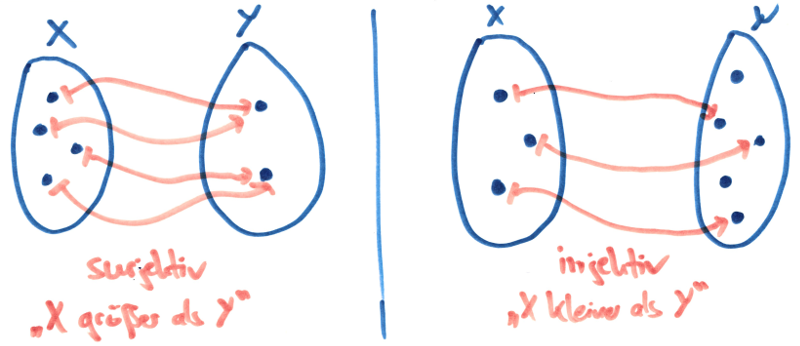
\includegraphics[width=0.8\textwidth]{images/groessenverhaeltnisse}
    \par}

    \pause
    Aber in~$\Eff(\STM)$ gibt es eine solche Injektion!
  }

  \only<3>{
    {\centering
    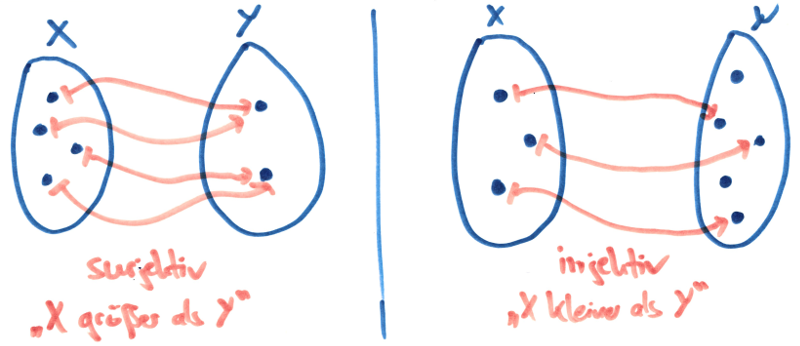
\includegraphics[width=0.7\textwidth]{images/groessenverhaeltnisse}
    \par}

    \explanation{$\Eff(\STM) \models \text{"`Es gibt eine Injektion~$\NN^\NN \to
    \NN$."'}$}{Es gibt eine Superturingmaschine, welche bei Eingabe einer
    Kodierung einer Superturingmaschine~$A$, welche eine Funktion~$\NN \to \NN$ berechnet,
    eine Zahl~$n(A)$ berechnet und aufs Band schreibt. Dabei darf nur dann~$n(A)
    = n(B)$ sein, wenn~$A$ und~$B$ dieselbe Funktion berechnen.}
  }

  \only<4>{
    \justifying
    Die Superturingmaschine
    \code{
      Lese die Kodierung einer Superturingmaschine~$A$ vom Band ein.
      Gehe nun alle natürlichen Zahlen~$n$ der Reihe nach durch und prüfe
      jeweils, ob die~$n$-te Superturingmaschine dasselbe Verhalten zeigt
      wie~$A$. Da~$A$ terminiert, ist das entscheidbar. Gebe die kleinste so
      gefundene Zahl~$n$ aus.
    }
    schreibt bei Eingabe einer Kodierung einer Superturingmaschine~$A$, welche
    eine Funktion~$\NN \to \NN$ berechnet, eine Zahl~$n(A)$ aufs Band. Dabei ist
    nur dann~$n(A) = n(B)$, wenn~$A$ und~$B$ dieselbe Funktion berechnen.
    \par
  }
\end{frame}

\end{document}

Ein Hoch auf Turingmaschinen
* Einfachheit
* Maschinelle Umsetzung klar
* Robustheit des Konzepts
* Äquivalenz zu anderen Modellen (aber nur für N --> N)
* Verbindungen zur Logik
* (aber: "TM sind nicht alles", siehe zum Beispiel R-Maschinen oder QTM)

Crashkurs Ordinalzahlen

Erste Schritte mit Superturingmaschinen
* Definition
* Beispielaufgaben
* Halteproblem
* Schwerere Aufgaben

Besondere Phänomene
* Ausbrechen aus Wiederholungen
* Lost Melody
* Abmessbare Ordinalzahlen

Effektiver Topos

"Allgemein sollten im Vortrag auch Maschinen vorgeführt werden, deren
Halteverhalten von mengentheoretischen Eigenschaften abhängt. Zum Beispiel die
Sache mit der Unabhängigkeit von BB(n) für kleine Wert von n von Adam Yedidia
und Scott Aaronson. http://www.scottaaronson.com/busybeaver.pdf"
